\item Toda la información de los clientes del segmento Consumer que realizaron una orden con modo de envío Second Class y que no viven en Nevada.

\begin{lstlisting}
consumidores = σ segment = 'Consumer' (customer)

pedidos = σ shipmode = 'Second Class' (orders)

clientes = σ state ≠ 'Nevada' (consumidores)

π customerid, customername, segment, country, city, state, postalcode, region
  (clientes ⨝ π customerid (pedidos))
\end{lstlisting}

\begin{center}
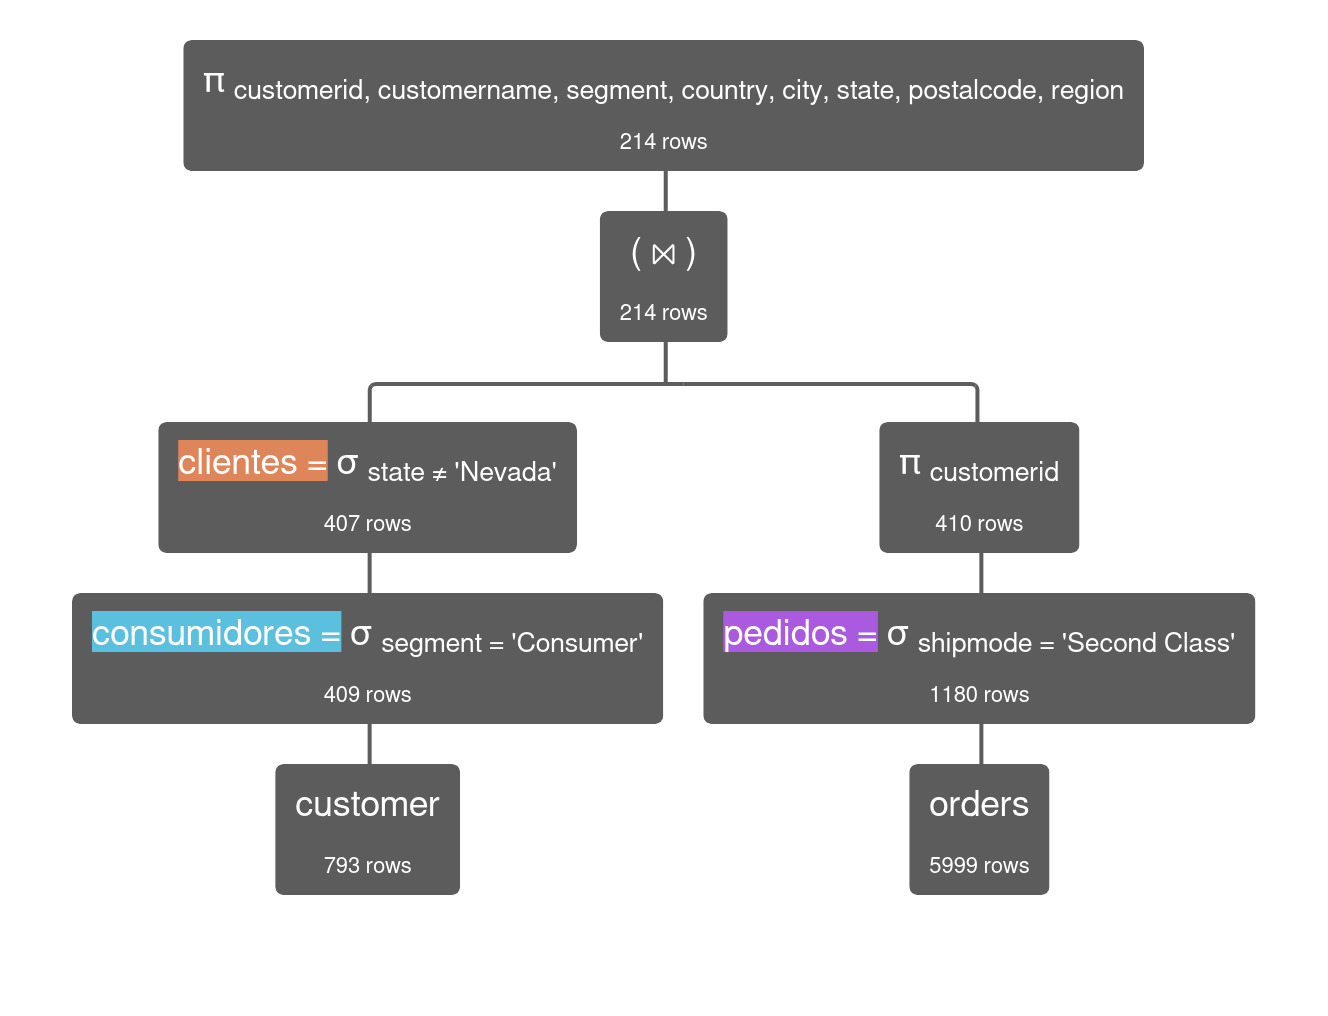
\includegraphics[width=0.75\textwidth]{figuras/2d_arbol.jpg}
\end{center}

\begin{center}
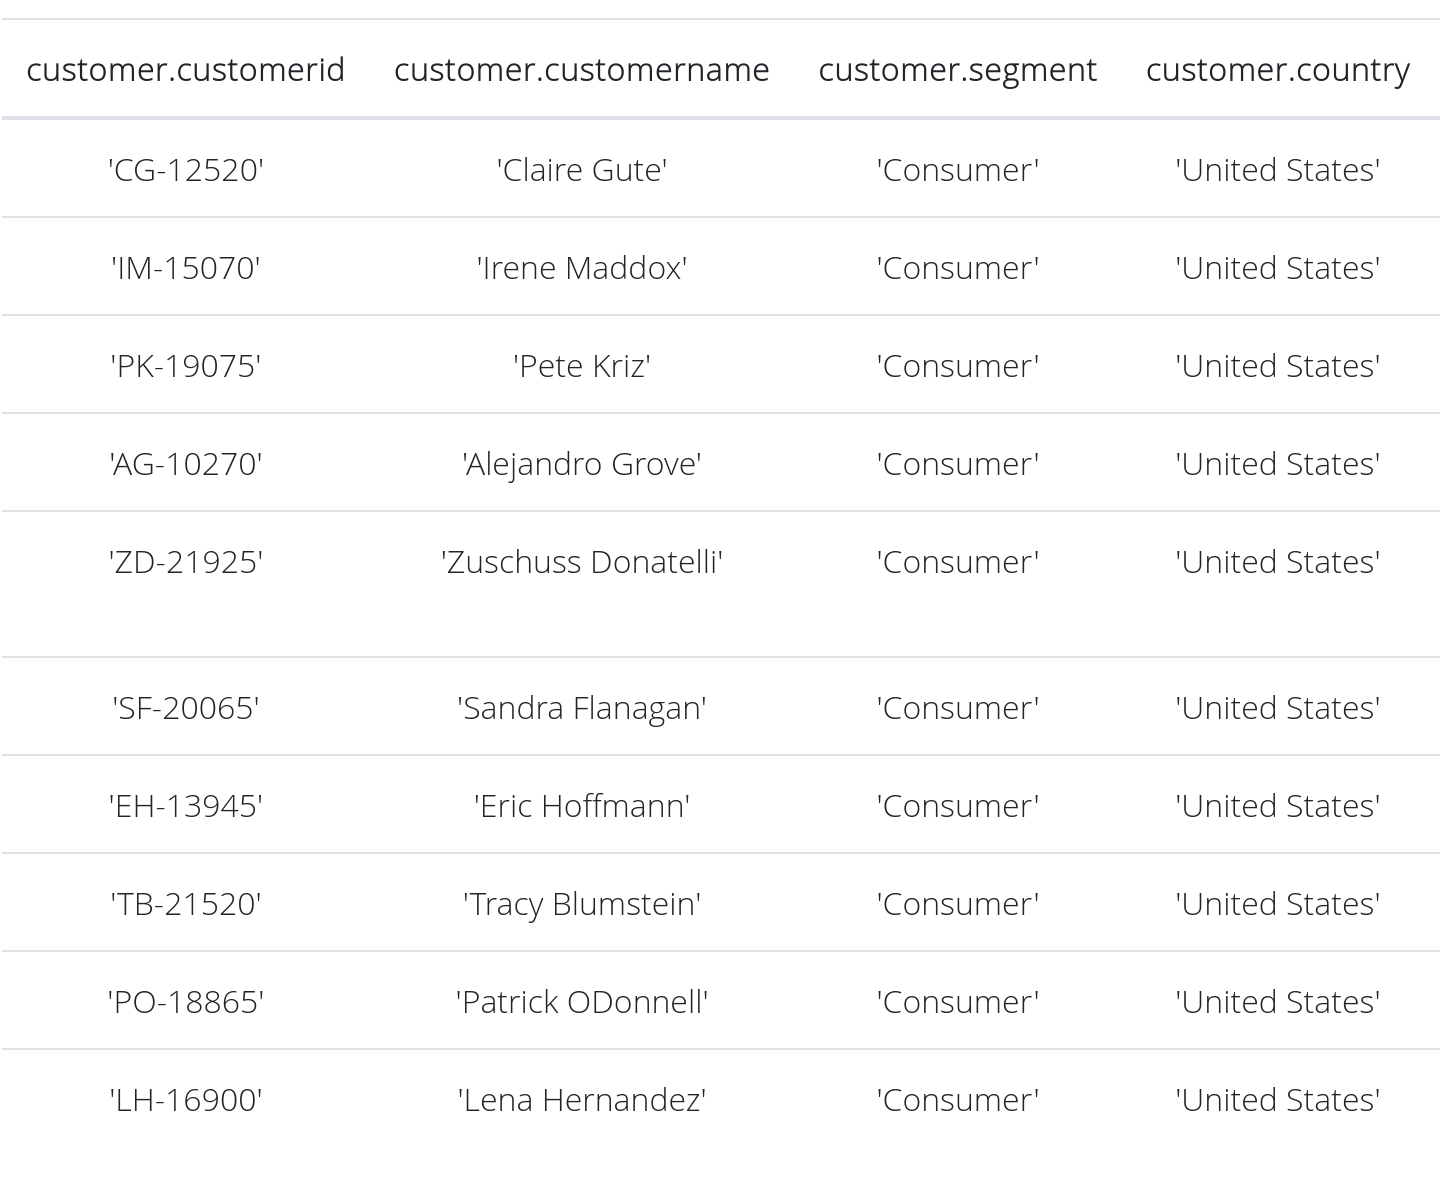
\includegraphics[width=0.4\textwidth]{figuras/2d_tuples.png}
\end{center}

\newpage
